\documentclass[a4paper,12pt]{report}

\usepackage{ort}
\usepackage[left=3cm,right=3cm,top=3cm,bottom=3cm]{geometry}

\usepackage[spanish, es-tabla]{babel}
\usepackage[below]{placeins}
\usepackage{fancyhdr}
\usepackage{graphicx}
\usepackage{enumerate}
\usepackage{blindtext}
\usepackage{listings}
\usepackage{etoolbox} 
\usepackage{titlesec}
\usepackage[utf8]{inputenc} 
\usepackage{graphicx}
\usepackage[table,xcdraw]{xcolor}
\usepackage{booktabs}
\graphicspath{ {imagenes/} }
\titleformat{\chapter}{\normalfont\huge\bf}{\thechapter.}{20pt}{\huge}


\title{Sistemas Operativos\\Obligatorio}
\author{Pablo Benitez - 179924\\Fabio Ramirez - 218566}
\usepackage{hyperref}
\hypersetup{pdfborder={0 0 0}}
\usepackage{float}

\begin{document}

\nocite{*}

\pagestyle{fancy}
\renewcommand\headrulewidth{0pt}
\fancyhf{}
\fancyfoot[R]{\thepage}

\fancypagestyle{plain}{
    \renewcommand{\headrulewidth}{0pt}
    \fancyhf{}
    \fancyfoot[R]{\thepage}
}

% Estilo Caso de Uso
\newcommand\tabularhead[1]{
\begin{table}[h]
 
  \begin{tabular}{|p{0.4\linewidth}|p{0.55\linewidth}|}
    \hline
    \textbf{Acción de los actores} & \textbf{Respuesta del Sistema} \\
    \hline}

  \newcommand\addrow[2]{#1 &#2\\ \hline}
  \newcommand\addmulrow[2]{ \begin{minipage}[t][][t]{2.5cm}#1\end{minipage}% 
     &\begin{minipage}[t][][t]{8cm}
      \begin{enumerate} #2   \end{enumerate}
      \end{minipage}\\ }

  \newenvironment{casodeuso}{\tabularhead}
{\hline\end{tabular}\end{table}}

\maketitle


\begin{abstract}
    Es aqui donde vendria el abstract. Cada chapter que se cree en el documento principal generará automaticamente una entrada en el indice asi como las section
    
\end{abstract}

\tableofcontents
\chapter{Obetivos o Introduccion}
    \pagenumbering{arabic}
    \section{SEccion 1}
    Para poder usar la maquina virtual "LAMP" que se encuentra en aulas, primero debemos descargar el programa VirtualBox desde \url{https://www.virtualbox.org/wiki/Downloads}.
    
    Luego tenemos que obtener la mencionada maquina virtual desde la web del curso, que se encuentra en \url{https://aulas.ort.edu.uy/course/view.php?id=3885&section=10} .
    Dependiendo de la arquitectura de su OS debe bajar el archivo de 32bits o 64bits.
    
    Descargada la VM(virtual machine) se debe agregar a la aplicación de VirtualBox, haciéndolo desde el menú o dándole doble click al archivo. Hecho esto se debería de ver como la siguiente imagen:
    \begin{figure} [H]
            \centering
            \frame{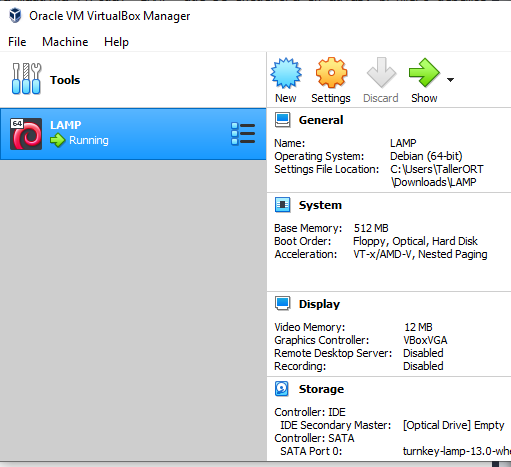
\includegraphics[width=4in]{imagen/vm1.png}}
            \caption{Inicio de VirtualBox}
    \end{figure}
    
    \clearpage
    Tenemos que iniciar LAMP con el botón de la flecha verde. Con esto nos cargara una pantalla donde se muestra el sistema operativo Linux iniciando, y al terminar nos mostrara la dirección ip que se usara para cada servicio.
    
    A continuación se despliega una muestra de como se vería:
    
    \begin{figure} [H]
            \centering
            \frame{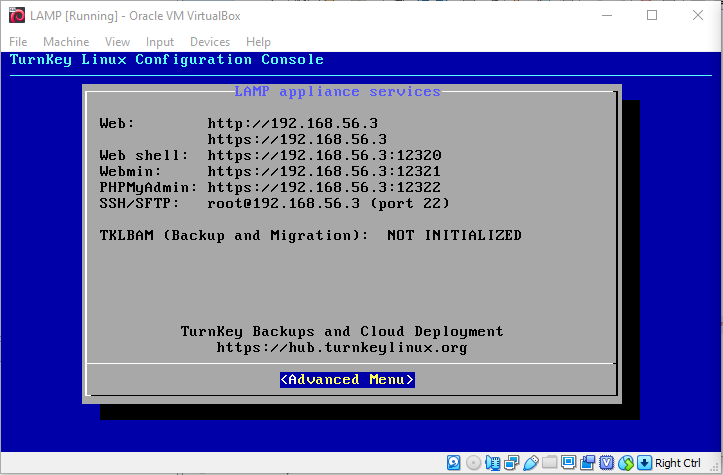
\includegraphics[width=4in]{imagen/vm2.png}}
            \caption{Maquina virtual corriendo}
    \end{figure}
    
    
    Con esta IP ya podemos acceder desde cualquier navegador a la configuracion tanto de la bases de datos en Mysql como del linux y dentro de este del servidor Apache con PHP.
    \clearpage
    Al acceder veremos lo siguiente:
    \begin{figure} [H]
            \centering
            \frame{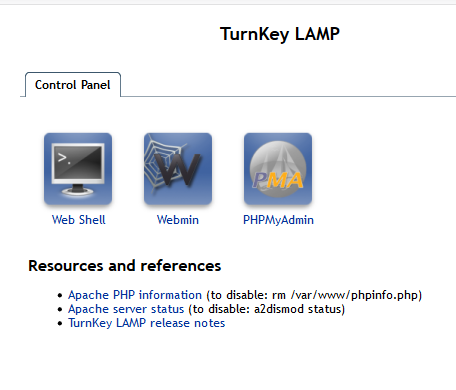
\includegraphics[width=4in]{imagen/IP.png}}
            \caption{Acceso por navegador}
    \end{figure}
    
    Tanto para acceder a la consola como al administrador de Mysql es necesario usar las credenciales: usuario= root, password = root.
    Si queremos acceder al Linux por otra via que no sea "Web Shell" también se puede usar putty. Lo mismo para subir archivos, podemos hacerlo con la app WinSCP.
    
\chapter{Fuentes}
    \pagenumbering{arabic}
    \section{Acceso a las fuentes}
    Todas las fuentes de este obligatorio están accesibles en
    \url{https://app.box.com/s/redahk46upihnq7uaryd1gdcpwt29c92}


\end{document}
